\begin{task}[
  title=Demonstrator: enriched teaching with Jupyter,
  id=teaching,
  lead=EP,
  PM=6, % EP: 3PM, UPSUD: 2PM, EuXFEL 1 PM
  wphases={0-48},
  partners={EGI,UIO,UPSUD,XFEL}
  ]

  \textbf{Context}

  As argued in Task~\taskref{ecosystem}{teaching-tools}, the Jupyter
  ecosystem offers a versatile environment which has been widely
  adopted in higher education in the recent years. École
  Polytechnique, Université Paris-Sud and other participants from this
  project have been early adopters (see the description of \site{EP}
  and \site{UPSUD}).

  \begin{figure}[ht!]\centering
  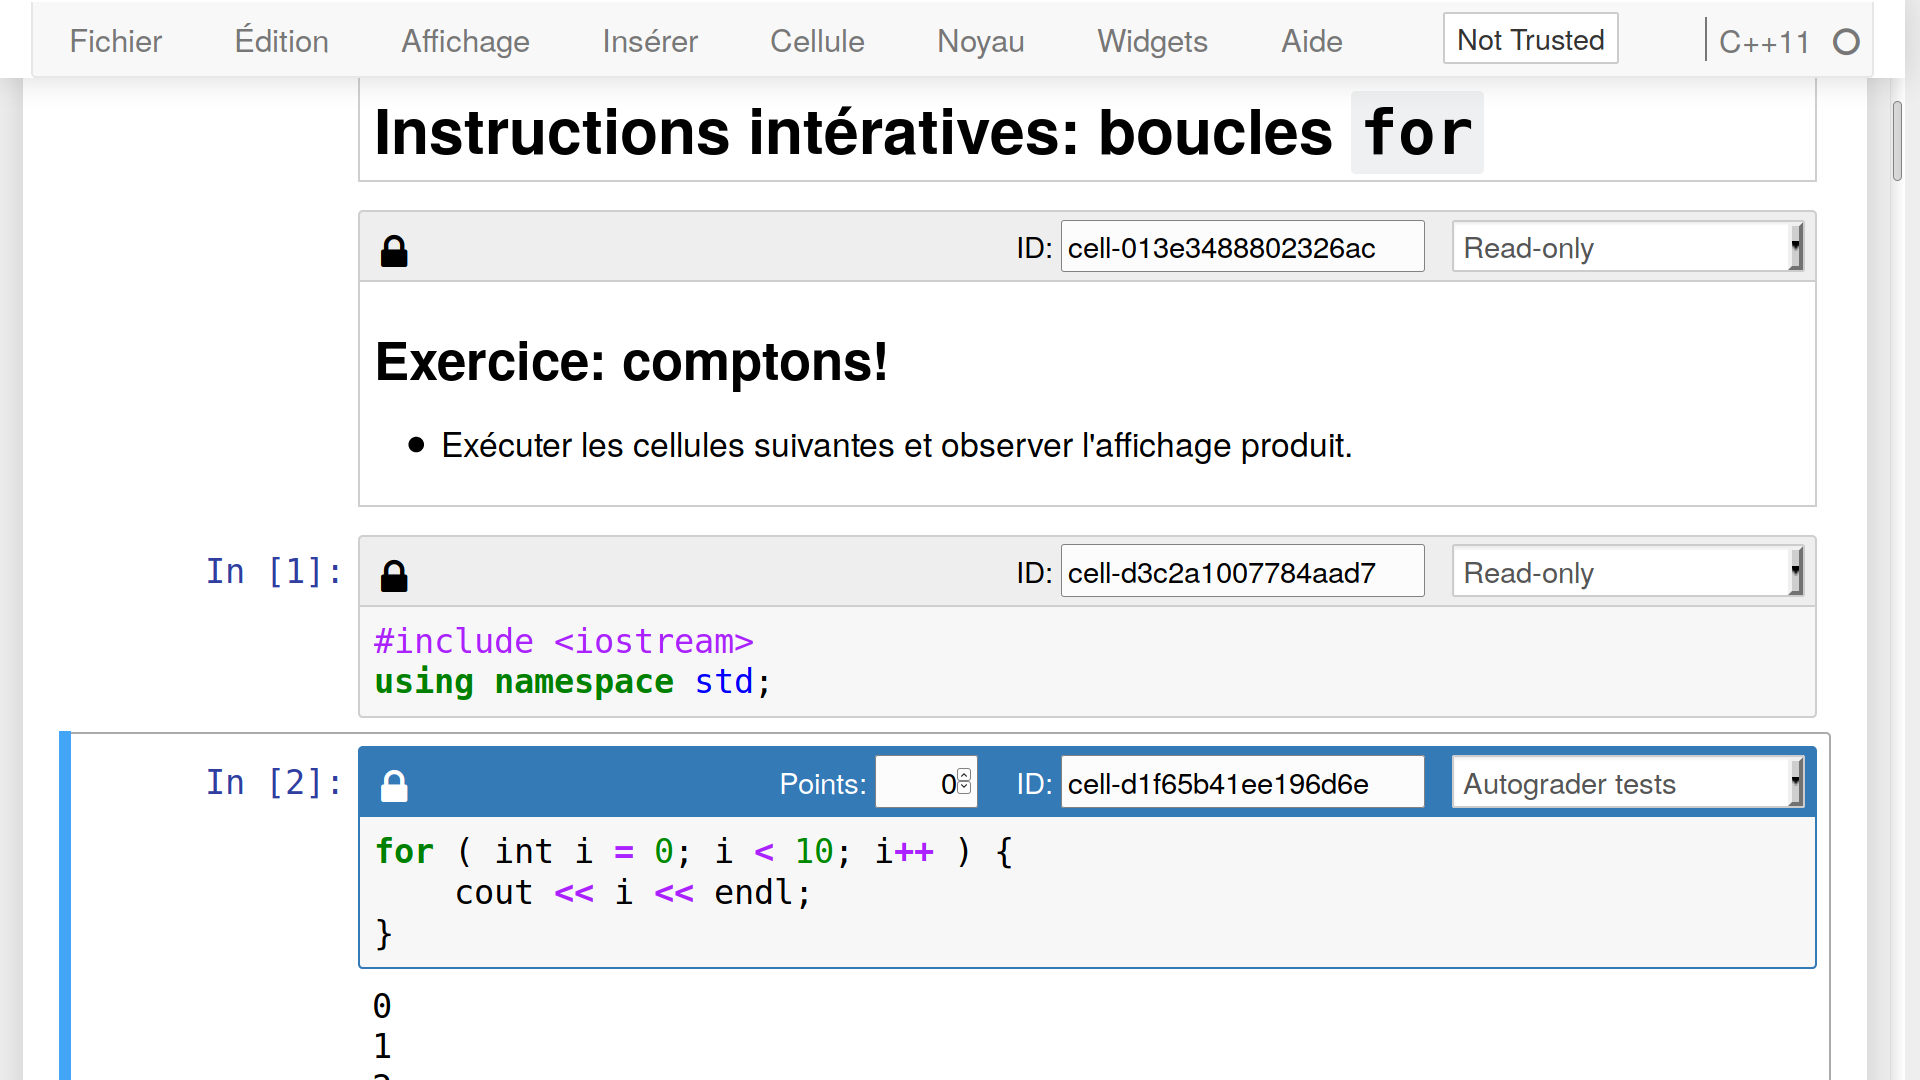
\includegraphics[width=.45\textwidth]{images/teaching-cling}\quad
  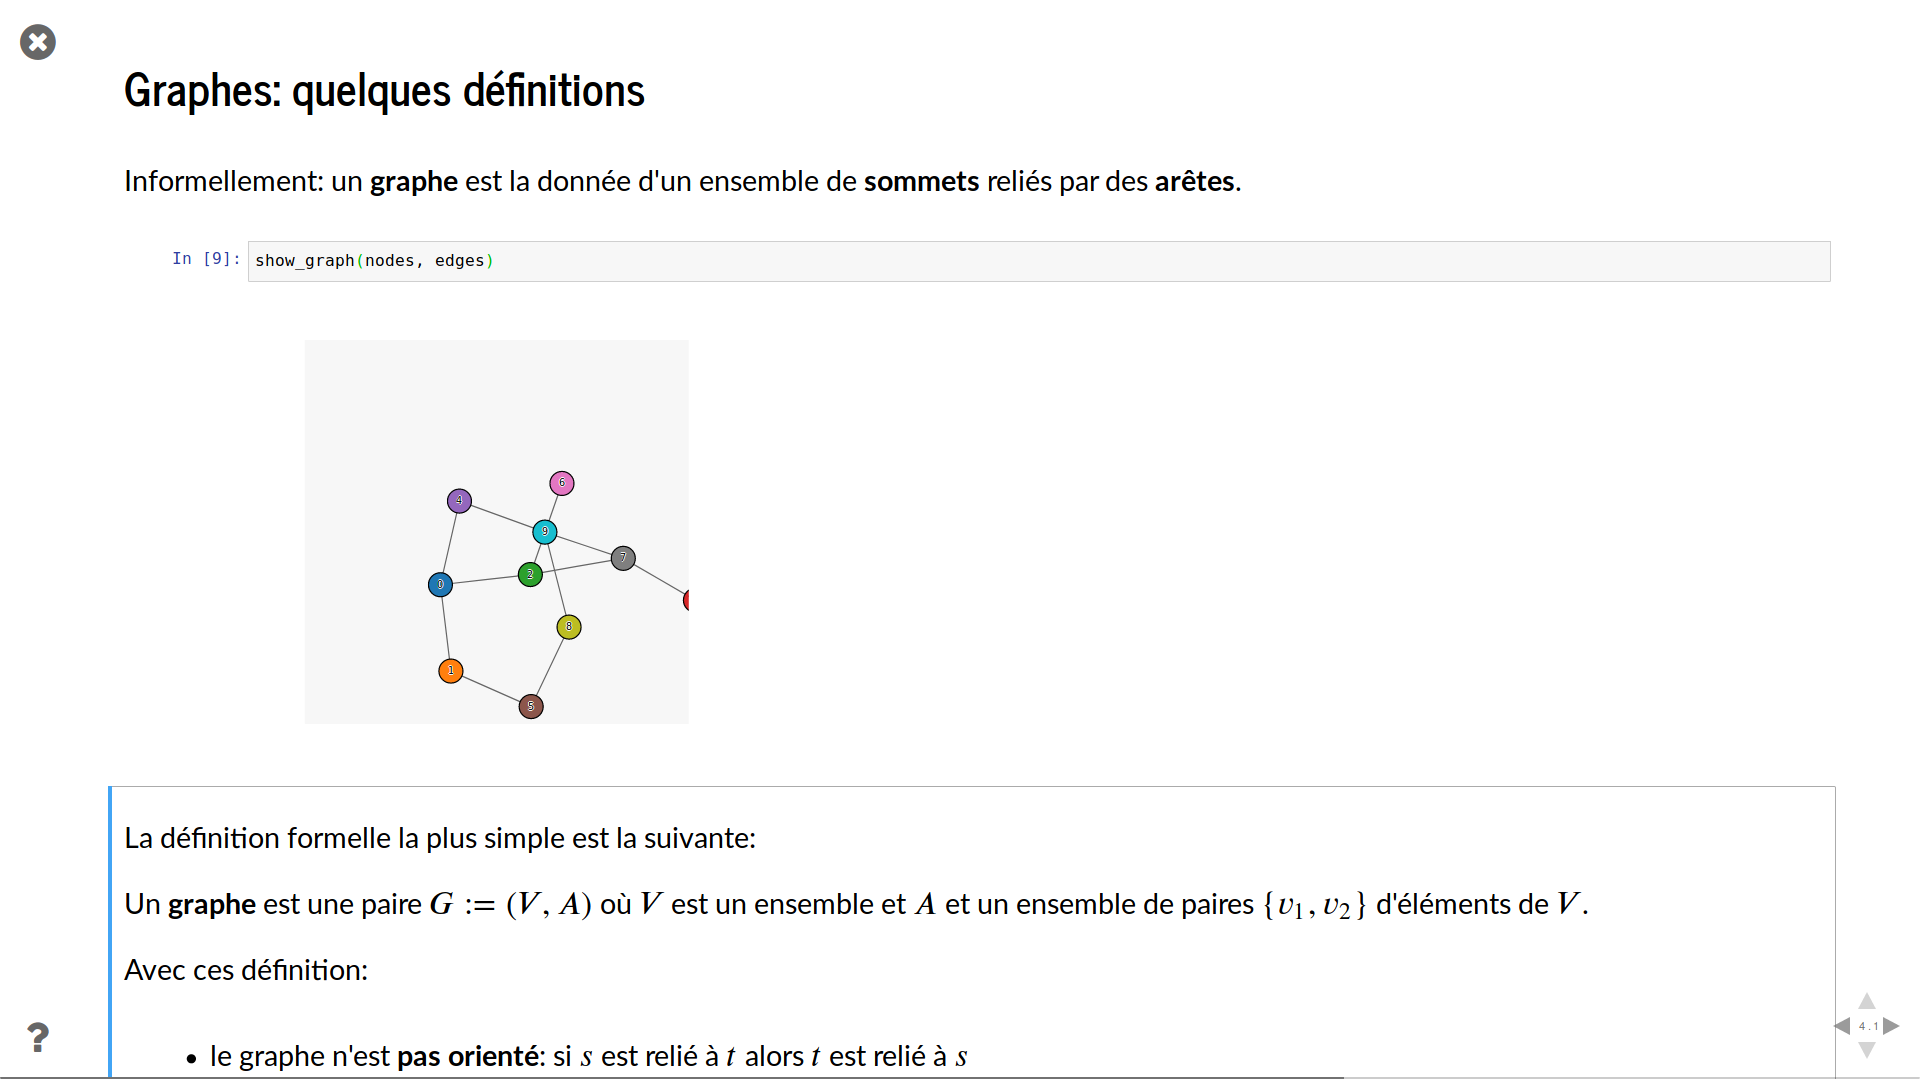
\includegraphics[width=.45\textwidth]{images/teaching-graphs}
  \caption{Jupyter based teaching material from Paris Sud. On the
    left: an exercise sheet for the course \emph{introduction to
      programming}; this instructor version showcases interactive C++
    execution and automatic grading configuration menus. On the right:
    interactive slides for a graph theory course.
    course.}\label{fig:teaching-cling}
  \end{figure}

  We learned the hard way that deploying the Jupyter environment at a
  large scale (e.g. for a university) requires specialized expertise
  (DevOps, software development, ...) which impediments its adoption
  by the greatest number of people. High quality hosted solutions
  (e.g. cocalc, gryd) do exist but are not the final solution when it
  is desired to get higher control on private data, integration with
  the local infrastructure (authentication, shared drive, e-learning
  environment, dedicated hardware, ...), or to use local computing
  resources rather than paid services.

  The following tasks will contribute to tackling those hurdles and
  offering better support for teaching:
  \begin{itemize}
  \item Tasks~\taskref{core}{jh-bh-conv}
    and~\taskref{eosc}{jh-bh-deployment} will greatly ease the
    deployment of Jupyter environments, with tight integration in the
    existing local infrastructure and full customizability by the
    teachers.
  \item Task~\taskref{ecosystem}{teaching-tools} will improve the
    interoperability with existing e-learning systems, and further
    develop teaching aids for, e.g., material sharing,
    (self)-evaluation, and grade management.
  \item Task~\taskref{applications}{math} will support teaching
    in mathematics through better support for real-time interactivity.
  \item Task~\taskref{ecosystem}{xeus-cpp} will support teaching
    in computer-science and scientific programming through
    better C++ integration in the notebook and will allow to first classe students to focus on the
    syntax of the language without distractions such as compiling and
    linking a program.
  \item Task~\taskref{eosc}{eosc} will ease publication and FAIR
    access to course material.
  \end{itemize}

  \textbf{This task}

  In this task, we will \textbf{deliver and help deliver Jupyter-based
    courses at a large scale} in our own institutions, as a mean to
  \textbf{inform, evaluate, provide feedback on, and demonstrate the
    value of the work performed} in this project in the context of
  higher education, as well as to \textbf{develop and share best
    practices} and \textbf{demonstrate and disseminate} Jupyter's full
  potential for teaching.

  \'Ecole polytechnique and Université Paris-Sud are particularly well
  suited for this task because they
  \begin{enumerate}
  \item host a variety of local infrastructure (dedicated servers,
    local cloud, computer labs, ...);
  \item host a reactive community with highly qualified research
    software engineers (DevOps, software developers), researchers,
    professors, and students that have been working together on this
    topic for several years, with close collaboration between the two
    sites;
  \item offer a diversity of courses, in many disciplines and ranging
    from large lower undergraduate courses to specialized classes for
    graduate students and top notch engineers;
  \item have strong support from their teaching departments.
  \item have an influential alumni structure through which the
    technology will be propagated.\TODO{do we want this item?}
  % \item will create a reactive community of students and researchers,
  %   where the dissemination of the project tools and experience will
  %   be easy, which will organize Jupyter days as in
  %   2018\footnote{\url{http://www.cmap.polytechnique.fr/~massot/Personal_web_page_of_Marc_Massot/JupyterX.html}}
  %   on a regular basis.
  \end{enumerate}

  % \TODO{HF: Loic, can you complete this, please?}

  % A variety of courses are delivered at Université Paris Sud using
  % Jupyter technologies. This includes for example programming classes
  % in C++ at lower undergraduate level (400 students per year since
  % 2017), a series of undergraduate and graduate math courses (computer
  % aided mathematics, computer algebra, numerical methods), or courses
  % in physics, bio-informatics, etc. To support these courses, a
  % JupyterHub service has been deployed in 2017 and progressively
  % improved since, on Paris Sud's local cloud infrastructure, enabling
  % students and teachers to work from anywhere and any device.

  % The Mathematics department at Ecole polytechnique has started a reform of their various teaching offer based on
  % Jupyter for two years and several courses of the Bachelor program, 2nd and 3rd
  % year of Engineering school and Master program have already begun relying on a
  % strong use of Jupyter notebooks / JupyterHub\footnote{MAP551 - 2nd yer course
  % MAP411 - AMS X02 - Mooc INRIA preciser?} and this will continue with a strong
  % support of the Dean of undergraduate studies and of graduate studies. Besides
  % several software and research engineers in applied mathematics have been
  % recruited and participate in this effort, as well as a administration engineer
  % in order to help in terms of building an infrastructure dedicated to Jupyter
  % with the support of the head of the Ecole polytechnique in order to disseminate
  % the effort into various other departments (Physics, Mechanical Engineering,
  % Biology...), where already some courses are starting based in Jupyter. The
  % link with the computer science club of students of Ecole polytechnique (Binet
  % R\'eseau) has also been created with the project and a community is emerging.

  The task includes the following activities
  \begin{compactitem}
  \item Reinforce the use of Jupyter technology in Courses at
    all levels, notably in Mathematics and Data Science, in close
    collaboration between Ecole polytechnique and Université Paris Sud;
  \item Test the new developments and feed back to tasks
    \taskref{core}{jh-bh-conv}, \taskref{ecosystem}{xeus-cpp}, \taskref{ecosystem}{teaching-tools}, \taskref{applications}{math} and \taskref{eosc}{jh-bh-deployment};
  \item Follow up on a successful Jupyter day in
    2018~\footnote{\url{http://www.cmap.polytechnique.fr/~massot/Personal_web_page_of_Marc_Massot/JupyterX.html}}
    by organizing a yearly Jupyter event showcasing the latest
    advances for teaching and research;
  \item Foster sharing of experience, best practices and course
    material, at the local level, and then worldwide, through meetups,
    blogs, etc.
  \end{compactitem}
  The outcome of this task will be reported on in \delivref{applications}{teaching}.
\end{task}
